\documentclass{book}
\usepackage{titling}
\usepackage{multirow}
\usepackage{setspace}
\usepackage{makeidx}
\usepackage{tikz}
\usepackage{subfigure}
\usepackage{braket}
\usepackage{graphicx}
\usepackage{array}

\usepackage{qcircuit}
\usepackage{graphicx}

\usepackage{tabularray}
\usepackage{amsmath}
\usepackage{circuitikz}
\usepackage{amssymb}
\usepackage{setspace}
\usepackage{amsmath}
\usepackage{xepersian}
\settextfont{XB Zar}
\linespread{1.5}



\makeatletter
\def\TikzBipolePath#1#2{\pgf@circ@bipole@path{#1}{#2}}
\def\CircDirection{\pgf@circ@direction}
\makeatother

% TikZ libraries `calc` needed now to tweak bracket.
\usetikzlibrary{backgrounds,fit,decorations.pathreplacing,calc}

\begin{document}
\tableofcontents
\section{مقدمه}	
در عصر حاضر بواسطه‌ی رشد و توسعه‌ی نظریه‌ی اطلاعات کوانتومی و سرمایه‌گذاری های مالی و انسانی بسیار در این زمینه،‌شاهد افزایش تعداد علاقمندان به این حوزه هستیم. در این پا .....

\section{comp vs superpos basis}

Chapter 1 chuang book

Consider the circuit shown in Figure 1.17, which applies Uf to an input not in the
computational basis. Instead, the data register is prepared in the superposition (|0〉 +
|1〉)/√2, which can be created with a Hadamard gate acting on |0〉. Then we apply Uf ,
resulting in the state:
% https://g.co/bard/share/2972a6a63b24



\chapter{آشنایی با مفاهیم اولیه}
\section{کیوبیت}

یک کیوبیت\footnote{Qubit}، معادل یک واحد اطلاعات کوانتومی می‌باشد. این مفهوم معادل مفهوم کلاسیک بیت\footnote{Binary Bit} می‌باشد. به طور کلی هر کیوبیت حاوی دو بیت اطلاعات است. برای تبیین یک کیوبیت از خصوصیات سامانه های کوانتومی، بهره‌می‌بریم. کیوبیت یک سیستم کوانتومی با فضای دوبعدی است. برای تعیین این دوبعد می‌توان ا ز یکی از خصویات سامانه های کوانتومی استفاده کرد. 

برخلاف بیت ها که مقادیر ثابت 0 یا 1 را به خود می‌گیرند؛ یک کیوبیت می‌تواند در یک حالت «برهمنهی کوانتومی» باشد؛ این بدان معناست که یک کیوبیت بواسطه‌ی مشاهده ناظر به یکی از حالات 0 یا یک تبدیل شود. این مهم‌ترین مزیت استفاده از کیوبیت‌هاست. بیان ریاضی یک کیوبیت ،در حالت برهمنهی، به شرح زیر است:
\vspace{2cm}
$$
\left\{
\begin{array}{ll}
	  \vert \psi \rangle = \alpha\vert 0 \rangle + \beta\vert 1 \rangle \\
	  \alpha^2 + \beta^2 = 1
\end{array}
\right.
$$
\vspace{2cm}

\newpage
کت‌ها$\vert 0 \rangle$ و $\vert 1 \rangle$ بیانگر پایه‌های فضای 
محاسباتی\footnote{\lr{Computational Basis Vectors}} هستند؛ و مقادیر $\alpha^2$ و $\beta^2$ بیانگر احتمال وقوع هر یک از این حالات، در صورت مشاهده، می‌باشند.

نمایش بردار $\psi$ به شرح زیر است:
\begin{center}
\begin{tikzpicture}
	
	% Define the axes
	\draw[->] (-2,0)--(2,0) node[right]{$\vert 0 \rangle$};
	\draw[->] (0,-2)--(0,2) node[above]{$\vert 1 \rangle$};
	
	% Draw the vector
	\draw[black,-stealth] (0,0)--(1,2) node[anchor=south west]{$\vec{\psi}$};
	
	% Label the components of the vector
	\node[below] at (1,0) {$$};
	\node[left] at (0,2) {$$};
	
\end{tikzpicture}
\end{center}

در بسیاری از مواقع برای سهولت در محاسبات، عملگر‌ها و حالات کوانتومی به کمک ماتریس‌ها نمایش داده ‌می‌شوند. فرم ماتریسی هر یک از حالات ذکر شده در بالا به شرح زیر است:

\begin{equation}
	\vert 1 \rangle = \begin{pmatrix} 0 \\ 1 \end{pmatrix}
	\hspace{2cm}
	\vert 0 \rangle = \begin{pmatrix} 1 \\ 0 \end{pmatrix}	
\end{equation}

برای تعریف کیوبیت ها، راه های زیادی وجود دارد، حالات قطبش فوتون،‌اسپین الکترون،‌یا سطوح انرژی اتم،‌هریک می‌توانند تعیین کننده‌ی بردار‌های فضای کیوبیت باشند.

\section{bloch vector - computayional basis - fourier basis}
\section{گیت‌های کوانتومی}
گیت‌های کوانتومی\footnote{\lr{Quantum Gates}} یکی از اولین و ههم‌ترین اجزای‌ مدار‌های کوانتومی ‌می‌باشند. این گیت‌ها عملگر‌هایی با قابلیت اثر‌گذاری روی کیوبیت‌ها می‌باشند. با اعمال یک گیت کوانتومی بر روی یک یا چند کیوبیت، می‌توان تغییرات مدنظر خود را روی کیوبیت اعمال کرد. با کمک این گیت‌ها می‌توان باعث برهم‌نهی کوانتومی یا رمز‌گذاری داده در داخل یک یا چند کیوبیت شد.

\subsection{انواع گیت کوانتومی}
گیت‌های کوانتومی، دارای انواع مختلف گوناگونی می‌باشند. به طور کلی گیت‌های کوانتومی، عملگر‌هایی یکه و بازگشت‌پذیر می‌باشند. 
\subsection*{گیت هادامارد}
مهم‌ترین گیت کوانتومی،‌گیت هادامارد\footnote{\lr{Hadamard gate}} است. با اعمال اثر این گیت روی یک کیوبیت، آن کیوبیت به‌یک حالت برهم نهی‌ کوانتومی‌ گذار‌ می‌کند. به عبارت دیگر هر یک از زیرحالات این حالت برهم‌نهی، با احتمال یکسانی قابل رخ دادن‌ هستند. 
\vspace{1cm}
$$
H\ket{0} = \frac{1}{\sqrt{2}} (\ket{0} + \ket{1})
\hspace{2cm}
H\ket{1} = \frac{1}{\sqrt{2}} (\ket{0} - \ket{1})
$$
\vspace{1cm}

این گیت کوانتومی‌ به صورت خطی روی یک دسته‌ کت اثر مي‌کند. نمایش ماتریسی این گیت‌کوانتومی به شرح زیر است:
\begin{center}
	\[
	H = \frac{1}{\sqrt{2}}
	\begin{pmatrix}
		1 & 1 \\
		1 & -1
	\end{pmatrix}
	\]
\end{center}





\begin{align*}
	H |0\rangle = l\frac{1}{\sqrt{2}} \begin{pmatrix} 1 & 1 \\ 1 & -1 \end{pmatrix} \begin{pmatrix} 1 \\ 0 \end{pmatrix} \
	= \frac{1}{\sqrt{2}} \begin{pmatrix} 1 \\ 1 \end{pmatrix} \
	= \frac{1}{\sqrt{2}} (|0\rangle + |1\rangle)
\end{align*}

\begin{align*}
	H |1\rangle = l\frac{1}{\sqrt{2}} \begin{pmatrix} 1 & 1 \\ 1 & -1 \end{pmatrix} \begin{pmatrix} 0 \\ 1 \end{pmatrix} \
	= \frac{1}{\sqrt{2}} \begin{pmatrix} 1 \\ -1 \end{pmatrix} \
	= \frac{1}{\sqrt{2}} (|0\rangle - |1\rangle)
\end{align*}

این گیت کوانتومی، یک گیت بازگشت‌پذیر است؛ یعنی اگر این گیت روی یک حالت کوانتومی اثر کند؛‌ می‌تواند آن را از حالت برهمنهی خارج کند. 

برای اعمال این گیت کوانتومی، فقط به یک کیوبیت نیاز داریم. به اصطلاح این گیت،‌یک \lr{Single-Qubit Quantum gate} می‌باشد.

نمایش این گیت‌کوانتومی در مدار با علامت زیر است:
\Qcircuit @C=1em @R=1.2em {
	& & \qw & \gate{H} & \qw \\
	& & & & \\
}


\subsection*{گیت CNOT}

گیت کوانتومی \lr{CNOT}\footnote{ controlled-NOT gate or controlled-X gate}، به عنوان گیت منطقی، یاد می‌شود. این گیت کوانتومی معادل گیت \lr{NOT} کلاسیک می‌باشد.
به‌طور معمول، برای اعمال اثر این گیت کوانتومی نیاز به دو کیوبیت داریم. این گیت کوانتومی فقط و فقط در مواقعی که «کیوبیت کنترل\footnote{Controled Qubit}» دارای مقدار $\vert 1 \rangle$ باشد، باعث تغییر وضعیت «کیوبیت هدف\footnote{Target Qubit}» می‌شود.

کیوبیت کنترل:
کیوبیت هدف:

خلاصه‌ای از عملکرد این تابع به شرح زیر است:\\
\textbf{ببین چرا از این نماد به جای تنسور پراداکت استفاده شده}
\begin{latin}
\begin{tabular}{ccccc}
	&&&&\\
	|A & B$\rangle$ &	&  |A &B $\oplus$ A $\rangle$  \\
	|control$\rangle$ & |target$\rangle$ & Effect CNOT Gate &|control$\rangle$ & |target$\rangle$ \\
	------- & -------- & -------- & -------- & --------  \\
	|0$\rangle$ & |0$\rangle$ & $\Longrightarrow$ &|0$\rangle$ & |0$\rangle$ \\
	|0$\rangle$ & |1$\rangle$ & $\Longrightarrow$ &|0$\rangle$ & |1$\rangle$ \\
	|1$\rangle$ & |0$\rangle$ & $\Longrightarrow$ &|1$\rangle$ & |0$\rangle$ \\
	|1$\rangle$ & |1$\rangle$ & $\Longrightarrow$ &|1$\rangle$ & |1$\rangle$
\end{tabular}
\end{latin}



نمایش ماتریسی این گیت کوانتومی به شکل زیر است:



اینا باید اصلاح بشه

$$
\text{CNOT} = \begin{pmatrix}
	1 & 0 & 0 & 0 \\
	0 & 1 & 0 & 0 \\
	0 & 0 & 0 & 1 \\
	0 & 0 & 1 & 0
\end{pmatrix}
$$



$$
\text{CNOT} \ket{1} = \begin{pmatrix}
	1 & 0 & 0 & 0 \\
	0 & 1 & 0 & 0 \\
	0 & 0 & 0 & 1 \\
	0 & 0 & 1 & 0
\end{pmatrix} \begin{pmatrix}
	1 \\
	0 \\
	0 \\
	0
\end{pmatrix} = \begin{pmatrix}
	0 \\
	0 \\
	0 \\
	1
\end{pmatrix} = \ket{1}
$$


$$
\text{CNOT} \ket{11} = \begin{pmatrix}
	1 & 0 & 0 & 0 \\
	0 & 1 & 0 & 0 \\
	0 & 0 & 0 & 1 \\
	0 & 0 & 1 & 0
\end{pmatrix} \begin{pmatrix}
	1 \\
	1 \\
	0 \\
	0
\end{pmatrix} = \begin{pmatrix}
	0 \\
	1 \\
	0 \\
	0
\end{pmatrix} = \ket{10}
$$
\vspace{2cm}

نمایش در داخل مدار:

\vspace{2cm}
\Qcircuit @C=1em @R=.7em {
	& \ctrl{1} & \targ & \qw \\
	& \targ & \ctrl{-1} & \qw
}

از این گیت کوانتومی‌، برای بسیاری مدار‌ها و شبیه‌سازی‌های کوانتومی، از جمله تلپورت، درهمتنیدگی و ...، استفاده می‌شود.





\subsubsection*{گیت توفولی}
گیت کوانتومی توفولی،‌یک نوع خاص از گیت \lr{CNOT} است. سازوکار این گیت مشابه گیت \lr{CNOT} می‌‌باشد؛‌ با این تفاوت که با در نظر گرفتن وضعیت دو کیوبیت کنترل شده، وضعیت کیوبیت سوم را تغییر می‌دهد. خلاصه ای از عملکرد این گیت کوانتومی به شرح زیراست:

به بیان دیگر اگر دو کیوبیت کنترل شده،‌ مقدار یک داشته باشند؛‌ کیوبیت هدف مقدارش تغییر می‌کند.
فرم ماتریسی این عملگر به شکل زیر است:

این گیت کوانتومی در مدار کوانتومی به شکل زیر نشان داده می‌شود:

\subsection*{گیت تغییر فاز}
گیت تغییر فاز\footnote{Phase shift gate}، یکی از گیت های مهم کوانتومی‌ می‌باشد. این گیت با ضرب کردن یک عدد ثابت در فاز یک کیوبیت، باعث تغییر فاز کیوبیت می‌شود. این گیت کوانتومی در بسیاری از الگوریتم‌های سرچ کوانتومی به‌کار می‌رود. این گیت بدین صورت تعریف می‌شود:

فرم ماتریسی این گیت به شرح زیر است:

این گیت کوانتومی در مدار کوانتومی به شکل زیر نشان داده می‌شود:

\subsection*{گیت دوران}
گیت دوران، \footnote{Rotation gate}، باعث دوران حالت کیوبیت، در فضای هیلبرت ‌می‌شود. پایه‌های فضای هیلبرت مذکور بردار های................................... هستند. نمایش این گیت کوانتومی به شرح زیر است:

فرم ماتریسی این گیت به شرح زیر است:
نمایش این گیت در مدار کوانتومی به شرح زیراست:


\subsection{Swap gate}

% https://www.youtube.com/watch?v=_p7i2v21Ys8&t=188s
% https://www.youtube.com/watch?v=F2okky5vD8k&list=PL1826E60FD05B44E4&index=11



\section{مدار‌های کوانتومی}

مدار‌های ‌کوانتومی\footnote{quantum circuit}، یک دسته از گیت ها‌ی کوانتومی،که با یک توالی بخصوص قرار گرفته اند، ‌می‌باشند. این کیوبیت ها، با توالی یاد شده، روی یک یا چند دسته کیوبیت، اثر داده ‌می‌شوند. 

مدار‌های کوانتومی، یکی از اولین مفهوم‌های بکار‌رفته برای تعریف کامپیوتر‌های کوانتومی‌ می‌باشند. برای تعریف و شبیه‌سازی هریک از پدیده‌ها و الگوریتم‌های کوانتومی، نیاز به یک مدار به‌خصوص داریم.

\subsubsection{شباهت ها و تفاوت های مدارهای کلاسیک و کوانتومی}
Quantum circuits are similar to classical circuits, but they use quantum gates instead of classical logic gates. Quantum gates are reversible operations that can be used to manipulate the quantum state of a qubit.

Sure, here are some similarities and differences between quantum circuits and classical circuits:

**Similarities:**

* Both quantum and classical circuits are composed of a sequence of operations that are applied to a set of data.
* Both circuits can be represented graphically using a similar notation.
* Both circuits can be used to implement algorithms.

**Differences:**

* Quantum circuits use qubits, which are quantum bits, as their basic unit of data. Classical circuits use bits, which are classical bits, as their basic unit of data.
* Quantum circuits use quantum gates, which are reversible operations, as their basic operations. Classical circuits use logic gates, which are irreversible operations, as their basic operations.
* Quantum circuits can exploit the properties of quantum mechanics, such as superposition and entanglement, to perform tasks that are impossible for classical computers.

Here is a table that summarizes the similarities and differences between quantum circuits and classical circuits:

| Feature | Quantum Circuit | Classical Circuit |
|---|---|---|
| Basic unit of data | Qubit | Bit |
| Basic operations | Quantum gates | Logic gates |
| Reversibility | Reversible | Irreversible |
| Exploits quantum mechanics | Yes | No |
| Possible tasks | Factoring integers, searching unsorted databases, simulating quantum systems | Sorting, calculating, logical operations |

I hope this helps! Let me know if you have any other questions.


\subsubsection{اجزای مدار‌های کوانتومی و سایز آن }
Operations: Operations are the actions that are performed on qubits. They can be measurements, initializations, or other actions.


The size of a quantum circuit is the number of gates in the circuit. The complexity of a quantum algorithm is often measured in terms of the size of the quantum circuit that is required to implement it.


Qubits

Qubits are the basic unit of information in quantum computing. They can be in a superposition of two states, 0 and 1. This means that a qubit can be both 0 and 1 at the same time, which is a property called quantum superposition. Qubits can also be entangled, which means that the state of one qubit is dependent on the state of another qubit.

Gates

Gates are operations that are applied to qubits. They can be used to create superpositions, perform rotations, and entangle qubits. There are many different types of gates, but some of the most common ones include the Hadamard gate, the CNOT gate, and the Toffoli gate.

Operations

Operations are the actions that are performed on qubits. They can be measurements, initializations, or other actions. Measurements are used to collapse the quantum state of a qubit into a definite value, 0 or 1. Initializations are used to set the state of a qubit to a specific value, 0 or 1.

Quantum Circuits

Quantum circuits are written using a graphical notation that is similar to the circuit diagrams used in classical computing. The horizontal axis of a quantum circuit represents time, and the vertical axis represents the qubits. The gates are represented by boxes, and the lines between the boxes represent the connections between the qubits.

Conclusion

The basic components of a quantum circuit are qubits, gates, and operations. These components are used to create quantum algorithms, which are algorithms that can only be performed on a quantum computer. Quantum circuits are a powerful tool for quantum computation, and they have the potential to revolutionize many different fields, including cryptography, chemistry, and machine learning.


\subsection{نحوه‌ی نمایش مدار‌های کوانتومی}

Quantum circuits are written using a graphical notation that is similar to the circuit diagrams used in classical computing. The horizontal axis of a quantum circuit represents time, and the vertical axis represents the qubits. The gates are represented by boxes, and the lines between the boxes represent the connections between the qubits.

Quantum circuits are a powerful tool for quantum computation. They can be used to implement a wide variety of quantum algorithms, including Shor's algorithm for factoring integers and Grover's algorithm for searching unsorted databases.

\chapter{برنامه‌نویسی کوانتومی}
\section{تفاوت کامپیوتر کلاسیک و کوانتومی}
\section{IBM Quantum computer and Qiskit}

\chapter{الگوریتم‌های‌کوانتومی‌}


چه گونه‌ای از مسائل محاسباتی قابل اجرا با مدارهای کوانتومی می‌باشند؟ 
تفاوت و برتری مدار‌های کوانتومی نسبت به مدار‌های کلاسیک چیست؟
آیا می‌توان یک حوزه‌ی خاص را تعیین کرد؛ به گونه‌ای که عملکرد کامپیوترهای‌‌کوانتومی نسبت به کامپیوتر‌های کلاسیک مزیت داشته باشند؟

در این بخش می‌خواهیم به طور خلاصه این سوالات را پاسخ دهیم و توضیح دهیم چگونه می‌توان از کامپیوتر‌های کوانتومی به شکلی سودمند استفاده کنیم.

\section{موازی سازی کوانتومی}

موازی‌سازی کوانتومی\footnote{Quantum parallelism}، پایه‌واساس بسیاری از الگوریتم‌های کوانتومی است. با گذار یک حالت کوانتومی به حالت برهمنهی کوانتومی، درحین محاسبات کوانتومی یک تابع نظیر \lr{f(x)}، می‌تواند مقادیر مختلف \lr{x} را به طور همزمان بررسی کند. این درحالیست که در محاسبات کلاسیک به دلیل ماهیت بیت‌های اطلاعات، تابع \lr{f(x)} فقط می‌تواند یکی از مقادیر مجاز برای \lr{x} را بررسی کند.


فرض کنید تابع f ،یک تابع تک-کیوبیت، به صورت زیر تعریف شده است:\\
\begin{center}
	$f (x) : \{0, 1\} \rightarrow \{0, 1\}$\\
\end{center}

روش مناسب برای محاسبه این تابع در یک کامپیوتر کوانتومی، با در نظر گرفتن دو کیوبیت که در حالت $\vert x, y\rangle$شروع می شود. با یک توالی مناسب از گیت های منطقی می توان این حالت را به $\vert f(x) \oplus x, y\rangle$ تبدیل کرد که در آن $\oplus$ بیانگر جمع مدوله با پایه‌2 می‌باشد.

\footnote{Modulo 2 is a mathematical operation that returns the remainder of a division by 2. For example, 5 mod 2 is 1, because 5 divided by 2 has a quotient of 2 and a remainder of 1.
	
	The symbol "⊕" is often used to indicate addition modulo 2. So, the expression "5 ⊕ 3" would be evaluated as follows:
	
	5 ⊕ 3 = (5 + 3) mod 2 = 8 mod 2 = 0
	This is because 8 divided by 2 has a quotient of 4 and a remainder of 0.
	
	Modulo 2 is a useful operation in many different areas of mathematics, including cryptography, computer science, and number theory. It is also used in everyday life, for example, when checking whether a number is even or odd.
	
	Here are some other examples of modulo 2:
	
	1 mod 2 = 1
	2 mod 2 = 0
	3 mod 2 = 1
	4 mod 2 = 0
	5 mod 2 = 1}

هریک از دسته‌های کیوبیت، \textbf{رجیستر کوانتومی} نامیده‌می‌شوند. اولین رجیستر، «رجیستر داده» و دومین رجیستر «رجیستر هدف» نامیده می‌شود.\\
ازین پس در این بخش به عامل گذار $\vert x, y \rangle \rightarrow \vert x, y \oplus f(x) \rangle$، عنوان «تابع \lr{$U_{f}$}» را اطلاق خواهیم کرد. لازم به ذکرست که این تبدیل، یک تبدیل یکه به شمار می‌آید.\footnote{اثبات این مطلب از حوصله‌ی بحث خارج است.}


اگر \lr{y = 0} آنگاه مقدار دومین کیوبیت بعد از اعمال تابع \lr{$U_{f}$} برابر با مقدار \lr{f(x)} خواهد بود.

 \begin{center}
 	 \begin{figure}[ht]
 		\centering
 		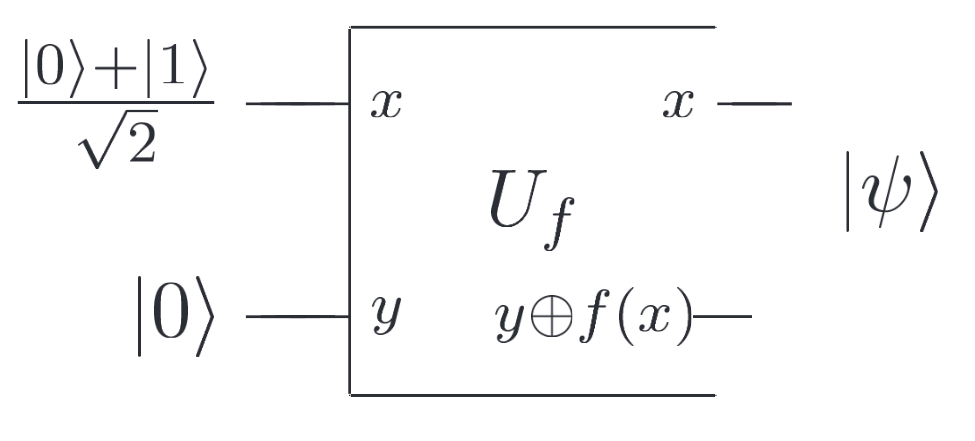
\includegraphics[width=0.8\textwidth]{Uforacle.png}
 		\caption{مدار کوانتومی برای ارزیابی $f (0)$ و $f (1)$ به طور همزمان. Uf مدار کوانتومی است که ورودی هایی مانند $\vert x, y\rangle$ را به $\vert x, y \rangle \rightarrow \vert x, y \oplus f(x) \rangle$، تصویر می‌کند.}
 	\end{figure}
 \end{center}

در شکل بالا مقادیر ورودی داده شده به تابع \lr{$U_{f}$} در پایه‌های محاسباتی قرار ندارند. رجیستر داده در حالت برهمنهی  قرار دارد. این حالت برهمنهی را می‌توان با اعمال گیت هادامارد بر حالت کوانتومی $\vert 0 \rangle$ ایجاد کرد. پس از ایجاد این حالت، تابع \lr{$U_{f}$} را به حالت جدید اعمال می‌کنیم:
\begin{center}
	$\frac{\vert 0,f(0) \rangle +\vert 1,f(1) \rangle }{\sqrt{2}}$
\end{center}

این یک حالت استثنایی است! جملات مختلف کسر بالا حاوی اطلاعاتی در مورد f (0) وf (1) می‌باشند؛ به‌نحوی که انگار f (x) را برای دو مقدار x به طور همزمان ارزیابی کرده ایم، این ویژگی به "موازی  سازی کوانتومی" موسوم می‌باشد. بر خلاف موازی سازی کلاسیک، که در آن هر یک مدارهای متعددی دارند ساخته شده برای محاسبه f (x) به طور همزمان اجرا می شوند، در اینجا برای ارزیابی تابع برای چندین مقدار x به طور همزمان، یک مدار f (x) (با قابلیت برهمنهی کوانتومی)استفاده می شود.

این فرآیند را می توان به راحتی  با استفاده از یک عمل کلی به نام تبدیل هادامارد، به توابعی با تعداد بیت دلخواه تعمیم داد. این عمل فقط تعداد n گیت هادامارد است که به طور موازی روی n کوبیت عمل می کنند.

برای مثال در شکل زیر؛ دو کیوبیت در حالت $\vert 0 \rangle$ آماده شده‌‌اند. پس از اعمال گیت‌های هادامارد بر روی این رجیستر به خروجی زیر خواهیم رسید: 

\begin{center}
	$ \Biggl( \frac{\vert 0 \rangle + \vert 1 \rangle}{\sqrt{2}}\Biggl)\Biggl( \frac{\vert 0 \rangle + \vert 1 \rangle}{\sqrt{2}}\Biggl) = \frac{\textbar00\rangle + \textbar01\rangle + \textbar10\rangle + \textbar11\rangle}{\sqrt{2}}$

\end{center}

از نماد $\operatorname{H} \otimes 2$ به عنوان نشانه‌ی عملکرد موازی دو گیت هادامارد استفاده می‌کنیم؛از علامت $\otimes$ به عنوان تانسور یاد می‌کنیم. به طور کلی نتایج اعمال موازی گیت هادامارد روی \lr{n} کیوبیت روی حالت کوانتومی برابرست با:

\begin{center}
	\[\frac{1}{\sqrt{2}} \sum_{x} \vert x \rangle\]
\end{center}


در اینجا، $\sum$ نشان دهنده جمع بر روی همه مقادیر ممکن \lr{x} است، و ما$\operatorname{H} \otimes n$  را برای نشان دادن این عمل می نویسیم.
اعمال تبدیل هادامارد روی یک بهمنهی کوانتومی برابر از همه حالت های محاسباتی تولید می کند؛ و با استفاده از فقط $n$ گیت، یک برهمنهی از $2n$ حالت تولید می کند.
\begin{center}
	\begin{figure}[ht]
		\centering
		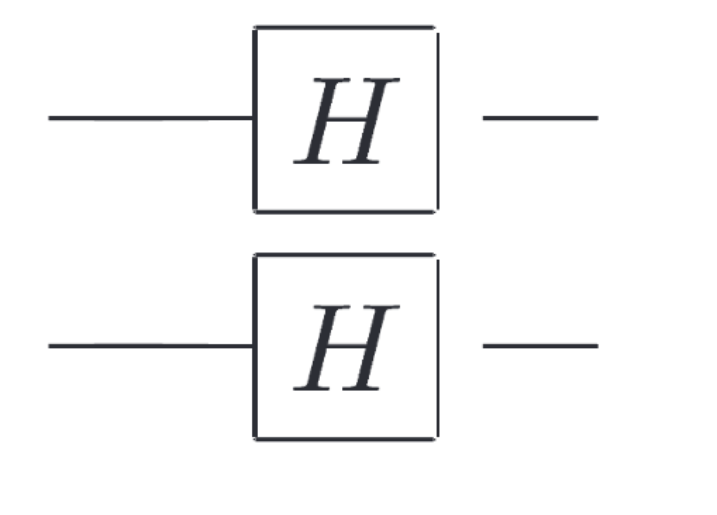
\includegraphics[width=0.8\textwidth]{Multyhadamard.png}
		\caption{اعمال تبدیل هادامارد $\operatorname{H} \otimes n$روی دو کیوبیت}
	\end{figure}
\end{center}

تبدیل هادامارد $\operatorname{H} \otimes 2$ روی دو بیت کوانتومی پیاده می‌شود. ارزیابی موازی کوانتومی یک تابع f(x) با ورودی n بیتی x و خروجی 1 بیتی، به روش زیر قابل پیاده‌سازی می‌باشد:

\begin{enumerate}
	\item ابتدا حالت $n + 1$ کیوبیت $\vert0\rangle^{\otimes n} \vert 0\rangle$ را آماده کنید،
	\item سپس تبدیل هادامارد را به $n$ کیوبیت اول و به دنبال آن مدار کوانتومی اعمال کنید.
	\item اعمال تابع $U_{f}$ به کیوبیت‌هایی که در حالت برهمنهی قرار دارند.
\end{enumerate}
درنهایت حالت زیر تولید ‌می‌شود:

1√2n∑x|x〉|f (x)〉

\begin{center}
	$\frac{1}{\sqrt{2^n}} \sum_{x} \vert x \rangle \vert f (x)\rangle$ 
\end{center}


به طور کلی موازی‌سازی کوانتومی امکان ارزیابی همزمان همه مقادیر ممکن تابع f را فراهم می‌کند، حتی اگر ظاهراً فقط یک بار f را ارزیابی کرده باشیم. با این حال، این موازی‌سازی بلافاصله مفید نیست. 


در مثال تک کوبیتی ما، اندازه‌گیری حالت فقط $\vert 0, f(0)\rangle$ یا $\vert 1, f(1)\rangle$ را می‌دهد! به طور مشابه، در حالت کلی، اندازه‌گیری حالت ∑x |x, f (x)〉 فقط$ f (x)$ را برای یک مقدار x خاص می‌دهد. البته یک کامپیوتر کلاسیک می‌تواند این کار را به راحتی انجام دهد! محاسبات کوانتومی برای مفید بودن به چیزی بیش از موازی‌سازی کوانتومی نیاز دارد؛ به توانایی استخراج اطلاعات مربوط به بیش از یک مقدار f (x) از حالت‌های سوپرپوزیسیون مانند ∑x |x, f (x)〉 نیاز دارد. 
در بخش های بعدی به مثال‌های خواهیم پرداخت که این مسائل را حل کند.



$\sum_{x} \vert x, f(x)\rangle$

\newpage
\subsection{مدل محاسباتی استاندارد}
پیش از بررسی مدل کوئری،‌ مدل ساده و استاندارد محاسباتی را بررسی می‌کنیم. به تصویر زیر دقت کنید:

\begin{figure}[ht]
	\centering
	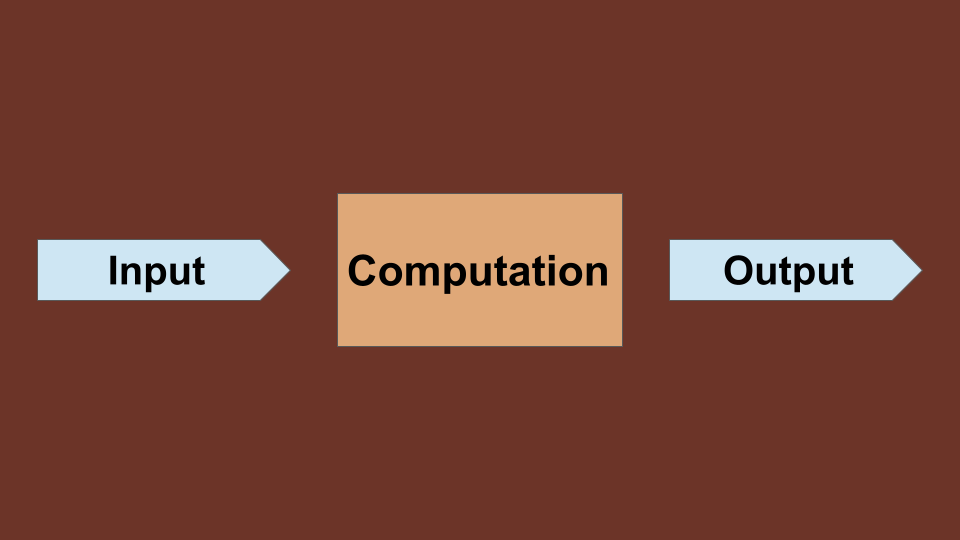
\includegraphics[width=0.8\textwidth]{standard computation model.png}
	\caption{یک واحد محاسباتی که مقادیری را به عنوان ورودی گرفته، پردازش کرده و سپس مقدار/مقادیر خروجی را ارائه کرده است.}
\end{figure}


در تصویر بالا یک نمود ساده از کامپیوتر‌های امروزی ارائه شده است. در دنیای واقعی مقدار ورودی می‌تواند از هر منبعی‌ تأمین شده باشد. با این وجود هدف ما بررسی منابع تولید ورودی نیست؛‌ بلکه هدف بررسی مقادیر ورودی (به صورت ایزوله) می‌باشد. می‌توان درنظر گرفت که ورودی داده شده و خروجی نهایی،‌هر دو در قالب یک رشته از اعداد باینری، ماتریس و یا هرقالب مدنظر کاربر باشند.

مهم‌ترین نکته درباره‌ی این واحد محاسباتی،‌ \textbf{در دسترس بودن کل مقادیر ورودی برای واحد پردازش} است. به عبارت دیگر\textbf{ واحد پردازش می‌تواند تمامی مقادیر ورودی را دریافت کرده و تشخیص} دهد. 

\section{مدل کوئری}
در مدل کوئری، داده‌های ورودی توسط یک تابع تولید می‌شوند. واحد محاسباتی دسترسی به تابع تولیدورودی دارد و می‌تواند برای دریافت داده‌های جدید،‌از تابع یاد شده،‌درخواست کند.

\begin{figure}[ht]
	\centering
	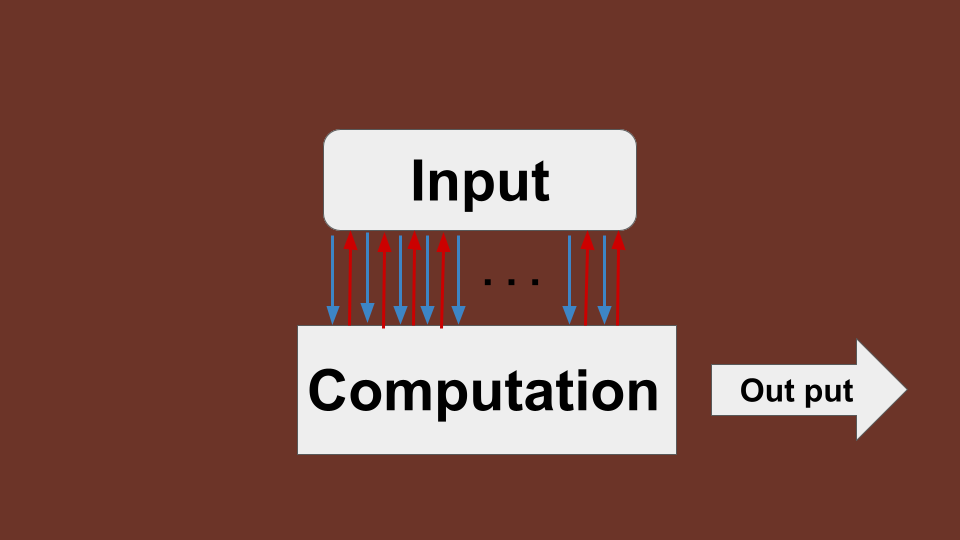
\includegraphics[width=0.8\textwidth]{Query computation model.png}
	\caption{شکل بالا نمود مدل محاسباتی‌کوئری است. واحد محاسباتی برای دریافت داده‌های جدید نیاز به درخواست از تابع \lr{input} دارد. خطوط قرمز و روبه‌بالا نشان از درخواست واحد محاسباتی و خطوط آبی روبه‌پایین نشان از پاسخ واحد \lr{input}می‌باشد.}
\end{figure}


در این مدل واحد محاسباتی دیگر داده‌ها را در قالب رشته‌ای از اطلاعات دردسترس ندارد؛ بلکه می‌تواند آن‌ها را از بخش \lr{input} دریافت کند. در گاهی از مواقع به سیستم \lr{input}،‌\lr{oracle} یا جعبه‌ی سیاه می‌گویند. تابع \lr{Oracle } یا جعبه‌ی سیاه یک سیستم است که ما به عنوان ناظر به سازوکار داخلی آن و  تمامی اطلاعات آن دسترسی نداریم و فقط می‌توانیم مقادیر مجاز را به آن داده و مقادیر خروجی را دریافت کنیم. 

تابع \lr{oracle} به صورت زیر تعریف می‌شود:
\begin{center}
$$
\left\{
\begin{array}{ll}
f : \sum^n = \sum^m\\
Which : m, n \in \mathbb{N}
\end{array}
\right.
$$
\end{center}

ما در این نظریه کوئری‌ها را می‌شماریم و وضعیت آن‌‌ها را بررسی می‌کنیم.

\section{معرفی و پیاده سازی الگوریتم دوچ}

\subsection{مسئله‌ی دوچ}
الگوریتم \lr{Deutsch} اولین و ساده‌ترین الگوریتم کوانتومی‌ است. این الگوریتم برای اولین بار در سال 1985 در مقاله‌ای مطرح شد؛ که توسط دیوید دوچ\footnote{David Deutsch} نوشته شده‌‌بود. این الگوریتم نقطه‌ی شروعی برای اثبات برتری کامپیوترهای کوانتومی نسبت به کامپوترهای کلاسیک است.

مسئله‌ی \lr{Deutsch} یکی از ساده‌ترین مفاهیم ممکن را مطرح می‌کند. اگر یک تابع به فرم زیر تعریف شود: 
\begin{center}
	$f : \sum \rightarrow \sum$
\end{center}
هدف بررسی ثابت بودن یا متعادل\footnote{Constante or balanse.} بودن تابع \lr{f} است. 
به‌طور کلی، درساده‌ترین حالت، می‌توان چهار وضعیت را برای تابع $f : \sum \rightarrow \sum$ درنظر گرفت:\\
\begin{figure}[ht]
	\centering
	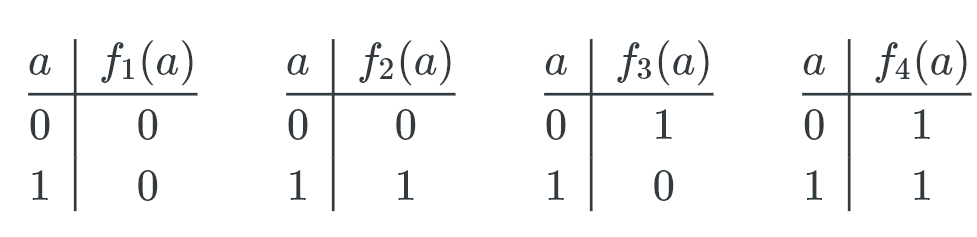
\includegraphics[width=0.8\textwidth]{Constantorbalanse.png}
	\caption{}
\end{figure}\\
در شکل بالا توابع \lr{f 1} , \lr{f 4} توابع ثابت و توابع \lr{f 2} و \lr{f 3} توابع متعادل هستند.
\begin{center}
\begin{tabular}{|c|c|}
	\hline
	\multicolumn{2}{|c|}{مسئله‌ی دوچ} \\
	\hline
	$f : \sum \rightarrow \sum$ & ورودی \\
	\hline
	صفر اگر تابع ثابت بود؛ یک اگر تابع متعادل بود.  & خروجی \\
	\hline
\end{tabular}
\end{center}
در الگوریتم‌های کلاسیک برای حل این مسئله، حداقل دو حالت باید بررسی شود.
\subsection{الگوریتم دوچ}
% quantum computer scinse : read it for yourself
% https://www.youtube.com/watch?v=2wticzHE1vs&t=2014s
% page 32

حال به بررسی الگوریتم دوچ می‌پردازیم. الگوریتمی که مسئله‌ی دوچ را با یک مدار کوانتومی حل می‌کند:\\
\begin{center}
\begin{figure}[ht]
	\centering
	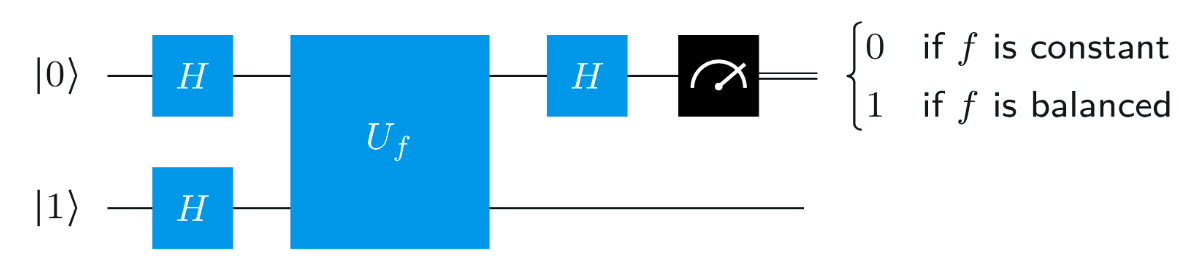
\includegraphics[width=0.8\textwidth]{Deutsch algorithm.png}
	\caption{}
\end{figure}
\end{center}

 
یک تغییر ساده در مدار شکل 1.3 نشان می دهد که چگونه مدارهای کوانتومی می توانند با پیاده سازی الگوریتم Deutsch از مدارهای کلاسیک پیشی بگیرند\footnote{ما در واقع یک نسخه ساده شده و بهبود یافته از الگوریتم اصلی را ارائه می دهیم.}. الگوریتم Deutsch ترکیبی از موازی سازی کوانتومی با خاصیتی از مکانیک کوانتوم به نام تداخل\footnote{how interference is using in deutsch algorithm : Interference is used in the Deutsch algorithm to distinguish between constant and balanced functions. A constant function is a function that always returns the same value, regardless of its input. A balanced function is a function that returns 0 for half of its inputs and 1 for the other half.
	
	The Deutsch algorithm works by first preparing two qubits in a superposition of states. The first qubit is prepared in the state |+⟩, which is the equal superposition of |0⟩ and |1⟩. The second qubit is prepared in the state |ψ⟩, which is a superposition of the states |0⟩ and |1⟩ with opposite phases.
	
	The two qubits are then passed through a quantum circuit that includes a Hadamard gate and a CNOT gate. The Hadamard gate transforms |+⟩ into the superposition |0⟩ + |1⟩, and the CNOT gate copies the state of the first qubit to the second qubit.
	
	After the quantum circuit has been executed, the two qubits are measured. If the first qubit is measured to be |0⟩, then the function f is constant. This is because the state |ψ⟩ is orthogonal to the state |0⟩, so the interference between the two states will destructively interfere.
	
	If the first qubit is measured to be |1⟩, then the function f is balanced. This is because the state |ψ⟩ is parallel to the state |1⟩, so the interference between the two states will constructively interfere.
	
	The Deutsch algorithm is a simple example of how quantum interference can be used to solve a problem that is difficult to solve classically. In this case, the Deutsch algorithm can distinguish between constant and balanced functions in a single step, while a classical computer would need to take an exponential number of steps.} است.
مشابه قبل،‌ابتدا از گیت هادامارد برای آماده سازی اولین کوبیت به عنوان superposition (|0〉 + |1〉)/√2 استفاده کنیم، اما اکنون کوبیت دوم y را با اعمال یک گیت هادامارد به حالت |1> به عنوان superposition (|0〉 - |1〉)/√2 آماده کنیم. به‌شکل زیر دقت کنید:



\begin{figure}[ht]
	\centering
	\includegraphics[width=0.8\textwidth]{Quantum circuit implementing Deutsch’s algorithm.png}
	\caption{پیاده‌سازی مدارکوانتومی‌ الگوریتم دوچ}
\end{figure}

\newpage

حالت ورودی:\\
\begin{center}
	$\vert\psi_{0}\rangle = \vert01\rangle$
\end{center}

سیستم دو کیوبیتی تشکیل شده،‌ پس از اعمال اثر دو گیت هادامارد می‌دهد:\\

\begin{center}
$\left|\psi_1\right\rangle=\left[\frac{|0\rangle+|1\rangle}{\sqrt{2}}\right]\left[\frac{|0\rangle-|1\rangle}{\sqrt{2}}\right]$
\end{center}
با کمی تأمل می‌توان دریافت که اگر Uf را به حالت |x〉(|0〉 - |1〉)/√2 اعمال کنیم، سپس به حالت (−1)f (x)|x〉(|0〉 - |1〉)/√2 می رسیم. بنابرین اعمال Uf به |ψ1〉 ما را با یکی از دو امکان زیر مواجه می کند:
\begin{center}
	$\left|\psi_2\right\rangle= \begin{cases} \pm\left[\frac{|0\rangle+|1\rangle}{\sqrt{2}}\right]\left[\frac{|0\rangle-|1\rangle}{\sqrt{2}}\right] & \text { if } f(0)=f(1) \\ \pm\left[\frac{|0\rangle-|1\rangle}{\sqrt{2}}\right]\left[\frac{|0\rangle-|1\rangle}{\sqrt{2}}\right] & \text { if } f(0) \neq f(1) \end{cases}$
\end{center}
با اعمال آخرین گیت هادامارد روی کیوبیت اول به حالت زیر خواهیم رسید:
\begin{center}
	$\left|\psi_3\right\rangle= \begin{cases} \pm|0\rangle\left[\frac{|0\rangle-|1\rangle}{\sqrt{2}}\right] & \text { if } f(0)=f(1) \\ \pm|1\rangle\left[\frac{|0\rangle-|1\rangle}{\sqrt{2}}\right] & \text { if } f(0) \neq f(1) \end{cases}$
\end{center}
با درنظر گرفتن شرایط زیر می‌توان $\vert\psi_{3}\rangle$ را به شکل زیر بازنویسی کرد:

$$
\begin{aligned}
	\left\{
	\begin{aligned}
		f(0) &= f(1) 
		\implies \qquad f(0) \oplus f(1) &= 0\\
		f(0) &\neq f(1) 
		\implies \qquad f(0) \oplus f(1) &= 1
	\end{aligned}
	\right.
\end{aligned}$$

از این رو:

\begin{center}
	$\left|\psi_3\right\rangle= \pm|f(0) \oplus f(1)\rangle\left[\frac{|0\rangle-|1\rangle}{\sqrt{2}}\right]$
\end{center}
بنابراین با اندازه گیری کیوبیت اول می توانیم $f(0) \oplus f(1)$ را تعیین کنیم. واقعاً جالب است! مدار کوانتومی به ما توانایی تعیین یک ویژگی جهانی از $f(x)$، یعنی$ f(0)\oplus f(1)$ را داده است، با استفاده از تنها یک ارزیابی از $f(x)$!این سریعتر از آن چیزی است که با یک دستگاه کلاسیک امکان‌پذیر است،یک دستگاه کلاسیک حداقل به دو ارزیابی نیاز دارد.
این مثال تفاوت بین موازی‌سازی کوانتومی و الگوریتم‌های تصادفی کلاسیک را برجسته می‌کند. به سادگی، ممکن است تصور شود که حالت $\vert0\rangle \vert f(0) \rangle + \vert1\rangle \vert f(1) \rangle$ مطابقت نزدیکی با یک رایانه کلاسیک تصادفی دارد که هرکدام از حالات $ f (0)$ یا$ f (1) $ با احتمال $1/2$ اندازه‌گیری می‌کند.
تفاوت این است که در یک رایانه کلاسیک این دو گزینه همیشه یکدیگر را حذف می‌کنند. در یک رایانه کوانتومی، امکان دارد که دو گزینه با یکدیگر تداخل داشته باشند تا برخی از خواص کلی تابع $f$ را با استفاده از چیزی شبیه به گیت هادامارد برای بازترکیب گزینه‌های مختلف، مانند آنچه در الگوریتم دوچ انجام شد، به دست آورند.
اساس طراحی بسیاری از الگوریتم‌های کوانتومی این است که یک انتخاب هوشمندانه از تابع و تبدیل نهایی اجازه می‌دهد تا اطلاعات جهانی مفیدی در مورد تابع تعیین شود - اطلاعاتی که نمی‌توان به سرعت در یک رایانه کلاسیک به دست آورد.

\section{الگوریتم دوچ - جوزا}
Deutsch’s algorithm is a simple case of a more general quantum algorithm, which we shall
refer to as the Deutsch–Jozsa algorithm. The application, known as Deutsch’s problem,
may be described as the following game. Alice, in Amsterdam, selects a number x from
0 to 2n − 1, and mails it in a letter to Bob, in Boston. Bob calculates some function
f (x) and replies with the result, which is either 0 or 1. Now, Bob has promised to use
a function f which is of one of two kinds; either f (x) is constant for all values of x,
or else f (x) is balanced, that is, equal to 1 for exactly half of all the possible x, and 0
for the other half. Alice’s goal is to determine with certainty whether Bob has chosen a
constant or a balanced function, corresponding with him as little as possible. How fast
can she succeed?

الگوریتم دوچ توضیح ساده از یک الگوریتم کوانتومی عمومی‌تر است که به عنوان الگوریتم دوچ-جوزا شناخته می‌شود. کاربرد این الگوریتم، که به عنوان مشکل دوچ شناخته می‌شود، به شرح زیر است:

آلیس، در آمستردام، یک عدد x را از بازه‌ $[0, 2^n-1]$ انتخاب می‌کند و آن را در یک نامه به باب، در بوستون، می‌فرستد. باب یک تابع$ f(x)$ را محاسبه می‌کند و نتیجه را که 0 یا 1 است، ارسال می‌کند. اکنون، باب قول داده است که از یک مدل تابع استفاده خواهد کرد؛ این تابع یا$ f(x)$ که برای همه مقادیر $x$ ثابت است، یا $f(x)$ متعادل است، یعنی‌ حاصل آن برای دقیقاً نیمی از همه xهای ممکن برابر با 1 است و برای نیمی دیگر برابر با 0 است.

هدف آلیس این است که با اطمینان و بکار بستن کمترین گام‌های ممکن تعیین کند که باب یک تابع ثابت یا متعادل را انتخاب کرده است. او چگونه می‌تواند به سرعت موفق شود؟

در حالت کلاسیک، آلیس ممکن است فقط یک مقدار x را در هر نامه به باب ارسال کند. در بدترین حالت، الی باید حداقل $\frac{2^n}{2} + 1$ بار از باب سوال کند، زیرا ممکن است قبل از دریافت یک، $\frac{2^n}{2}$ مرتبه پاسخ $0$ را دریافت کند. آلیس باید یک را دریافت کند؛‌تا بتواند به او بگوید که تابع باب متعادل است. 

یعنی در بهترین الگوریتم کلاسیک که می تواند استفاده کند بنابراین به$\frac{2^n}{2} + 1$ پرسش نیاز دارد. توجه داشته باشید که در هر نامه، آلیس n بیت اطلاعات را به باب ارسال می کند. علاوه بر این، در این مثال، فاصله فیزیکی باب و آلیس و به تبع آن افزایش هزینه محاسبه $f(x)$ و دشواری‌های احتمالی اجرای تابع $f(x)$ درنظر گرفته نشده‌است.

	اگر باب و آلیس بتوانند کوبیت ها را به جای بیت های کلاسیک مبادله کنند، و اگر باب موافقت کند $f (x)$ را با استفاده از تبدیل یکه‌ی \lr{$U_{f}$} محاسبه کند، سپس آلیس می تواند هدف خود را در یک مکاتبه با باب و با استفاده از الگوریتم زیر به دست آورد.
	
	با توجه به الگوریتم دوچ، آلیس یک رجیستر n کوبیتی را برای ذخیره پرس و جو خود آماده می کند و یک رجیستر کوبیت واحد را که به باب می دهد تا پاسخ را در آن ذخیره کند. او هر دو رجیستر پرس و جو و پاسخ خود را در یک حالت برهمنهی آماده می کند. باب f(x) را با استفاده از موازی سازی کوانتومی ارزیابی می کند و نتیجه را به آلیس برمی گرداند. آلیس سپس با استفاده از اعمال تبدیل هادامارد روی رجیستر پرس و جو(n-کیوبیتی)، حالات برهمنهی تداخل می‌دهد و با انجام یک اندازه گیری مناسب، تعیین می کند که آیا f ثابت یا متعادل است.
		
	گام‌های خاص الگوریتم در شکل 1.20 نشان داده شده است. بیایید با دنبال کردن این مدار، به بررسی حالات ایجاد شده بپردازیم.
	حالت ورودی |ψ0〉 = |0〉⊗n|1〉 (1.46)؛‌ شبیه حالت معادله (1.41) است، اما در اینجا رجیستر پرس و جو وضعیت n کوبیت را توصیف می‌کند که همه در حالت |0〉 آماده شده‌اند. پس از اعمال تبدیل هامادارد روی رجیستر پرس و جو  و روی رجیستر پاسخ، می‌توان نوشت:
	
	|ψ1〉 = ∑x∈{0,1}n|x〉√2n[ |0〉 − |1〉√2]
	
	
	
	The query register is now a superposition of all values, and the answer register is in an evenly weighted superposition of 0 and 1. Next, the function f is evaluated (by Bob)
	using Uf : |x, y〉 → |x, y ⊕ f (x)〉, giving (1.48) Alice now has a set of qubits in which the result of Bob’s function evaluation is stored
	in the amplitude of the qubit superposition state. She now interferes terms in the super-
	position using a Hadamard transform on the query register. To determine the result of
	the Hadamard transform it helps to first calculate the effect of the Hadamard transform
	on a state |x〉. By checking the cases x = 0 and x = 1 separately we see that for a single
	qubit H|x〉 = ∑
	z (−1)xz |z〉/√2. Thus (1.49) This can be summarized more succinctly in the very useful equation(1.50) where x · z is the bitwise inner product of x and z, modulo 2. Using this equation
	and (1.48) we can now evaluate |ψ3〉,(1.51) Alice now observes the query register. Note that the amplitude for the state |0〉⊗n is
	∑
	x(−1)f (x)/2n. 
	
	
	رجیستر پرس و جو اکنون یک برهمنهی از همه مقادیر ممکن به‌شمار می‌آید؛ درحالی که رجیستر پاسخ در یک برهمنهی به طور مساوی وزن شده از 0 و 1 محسوب می‌شود\footnote{یعنی احتمال رخ‌دادن صفر و یک یکسان است.}.
	
در مرحله بعد، تابع f توسط باب و به شکل Uf : |x, y〉 → |x, y ⊕ (x)〉f  ارزیابی می شود ، که (1.48) را می دهد.
	
	آلیس اکنون یک مجموعه کوبیت دارد که در آن نتیجه اعمال تابع باب در دامنه کوبیت حالت برهمنهی ذخیره می شود. او اکنون با استفاده از تبدیل هادامارد روی رجیستر پرس و جو، عبارات را در حالت برهمنهی کوانتومی تداخل می کند.
	
	برای تعیین نتیجه تبدیل هادامارد، بهترست ابتدا اثر تبدیل هادامارد را روی یک حالت |x〉 محاسبه کنیم. با بررسی موارد x = 0 و x = 1 به صورت جداگانه می بینیم که برای یک کوبیت واحد H|x〉 = ∑z (−1)xz |z〉/√2 می‌باشد. بنابراین (1.49)
	
	این را می توان به طور خلاصه در معادله بسیار مفید زیر خلاصه کرد:
	
	(1.50)
	
	جایی که x · z bitwise inner product x و z است، به modulo 2.
	
	با استفاده از این معادله و (1.48) اکنون می توانیم |ψ3〉 را ارزیابی کنیم:
	
	(1.51)
	
	آلیس اکنون رجیستر پرس و جو را مشاهده می کند. توجه داشته باشید که دامنه برای حالت |0〉⊗n است
	∑
	x(−1)f (x)/2n.
	
	
	
	
	
	\textbf{از استاد بپرس اشکاااااللللل}
	
	Let’s look at the two possible cases – f constant and f balanced – to
	discern what happens. In the case where f is constant the amplitude for |0〉⊗n is +1 or
	−1, depending on the constant value f (x) takes. Because |ψ3〉 is of unit length it follows
	that all the other amplitudes must be zero, and an observation will yield 0s for all qubits
	in the query register. If f is balanced then the positive and negative contributions to the
	amplitude for |0〉⊗n cancel, leaving an amplitude of zero, and a measurement must yield
	a result other than 0 on at least one qubit in the query register. Summarizing, if Alice measures all 0s then the function is constant; otherwise the function is balanced. The
	Deutsch–Jozsa algorithm is summarized below.
	
	
	بیایید به دو مورد ممکن - f ثابت و f متعادل - نگاه کنیم تا ببینیم چه اتفاقی می افتد.
	
	در صورتی که f ثابت باشد، دامنه برای حالت |0〉⊗n برابر است با +1 یا −1، بسته به مقدار ثابت f (x) که می‌گیرد.
	
	از آنجایی که |ψ3〉 طول واحد است، نتیجه می‌گیریم که تمام دامنه‌های دیگر باید صفر باشند، و یک مشاهده 0 را برای همه کوبیت‌ها در رجیستر پرس و جو به همراه خواهد داشت.
	
	اگر f متعادل باشد، سهم مثبت و منفی دامنه برای |0〉⊗n خنثی می‌شود، و یک دامنه صفر باقی می‌ماند، و یک اندازه‌گیری باید نتیجه‌ای غیر از 0 را در حداقل یک کوبیت در رجیستر پرس و جو به همراه داشته باشد.
	
	به طور خلاصه، اگر الی همه 0 را اندازه گیری کند، تابع ثابت است؛ در غیر این صورت تابع متعادل است.
	
	الگوریتم Deutsch-Jozsa در زیر خلاصه شده است:
	
	
	
	
	
	Algorithm: Deutsch–Jozsa
	Inputs: (1) A black box Uf which performs the transformation
	|x〉|y〉 → |x〉|y ⊕ f (x)〉, for x ∈ {0, . . . , 2n − 1} and f (x) ∈ {0, 1}. It is
	promised that f (x) is either constant for all values of x, or else f (x) is balanced,
	that is, equal to 1 for exactly half of all the possible x, and 0 for the other half.
	Outputs: 0 if and only if f is constant.
	Runtime: One evaluation of Uf . Always succeeds.
	Procedure:
	1. |0〉⊗n|1〉 initialize state
	2. → 1
	√2n
	2n −1∑
	x=0
	|x〉
	[ |0〉 − |1〉
	√2
	] create superposition using
	Hadamard gates
	3. → ∑
	x
	(−1)f (x)|x〉
	[ |0〉 − |1〉
	√2
	]
	calculate function f using Uf
	4. → ∑
	z
	∑
	x
	(−1)x·z+f (x)|z〉
	√2n
	[ |0〉 − |1〉
	√2
	]
	perform Hadamard transform
	5. → z measure to obtain final output z
	We’ve shown that a quantum computer can solve Deutsch’s problem with one evalu-
	ation of the function f compared to the classical requirement for 2n/2 + 1 evaluations.
	This appears impressive, but there are several important caveats. First, Deutsch’s prob-
	lem is not an especially important problem; it has no known applications. Second, the
	comparison between classical and quantum algorithms is in some ways an apples and
	oranges comparison, as the method for evaluating the function is quite different in the
	two cases. Third, if Alice is allowed to use a probabilistic classical computer, then by
	asking Bob to evaluate f (x) for a few randomly chosen x she can very quickly determine
	with high probability whether f is constant or balanced. This probabilistic scenario is
	perhaps more realistic than the deterministic scenario we have been considering. Despite
	these caveats, the Deutsch–Jozsa algorithm contains the seeds for more impressive quan-
	tum algorithms, and it is enlightening to attempt to understand the principles behind its
	operation.
	الگوریتم: Deutsch–Jozsa
	ورودی‌ها: (1) یک جعبه سیاه Uf که تبدیل زیر را انجام می‌دهد
	|x〉|y〉 → |x〉|y ⊕ f (x)〉, برای x ∈ {0، ...، 2n - 1} و f (x) ∈ {0، 1}. قول داده شده است که f (x) برای همه مقادیر x ثابت است یا f (x) متعادل است،
	یعنی برای دقیقاً نیمی از همه xهای ممکن برابر با 1 و برای نیمی دیگر 0 است.
	خروجی: 0 اگر و فقط اگر f ثابت باشد.
	زمان اجرا: یک ارزیابی Uf. همیشه موفق می شود.
	روش:
	
	|0〉⊗n|1〉 حالت را initialize کنید
	→ 1 √2n 2n −1∑ x=0 |x〉 [ |0〉 − |1〉 √2 ] ایجاد superposition با استفاده از دروازه‌های Hadamard
	→ ∑ x (−1)f (x)|x〉 [ |0〉 − |1〉 √2 ] تابع f را با استفاده از Uf محاسبه کنید
	→ ∑ z ∑ x (−1)x·z+f (x)|z〉 √2n [ |0〉 − |1〉 √2 ] تبدیل Hadamard را انجام دهید
	→ z اندازه گیری کنید تا خروجی نهایی z را بدست آورید ما نشان داده‌ایم که یک کامپیوتر کوانتومی می‌تواند مشکل Deutsch را با یک ارزیابی حل کند – ارزشیابی تابع f در مقایسه با نیاز کلاسیک برای 2n/2 + 1 ارزیابی. این به نظر چشمگیر است، اما چند نکته مهم وجود دارد. اول، مشکل Deutsch نیست یک مشکل مهم است؛ هیچ کاربرد شناخته شده ای ندارد. دوم، مقایسه بین الگوریتم های کلاسیک و کوانتومی تا حدودی مقایسه سیب و پرتقال است، زیرا روش برای ارزیابی تابع در دو مورد بسیار متفاوت است. سوم، اگر آلیس مجاز باشد از یک کامپیوتر کلاسیک احتمالی استفاده کند، سپس با درخواست از باب برای ارزیابی f (x) برای چند x به صورت تصادفی می تواند بسیار سریع تعیین کند با احتمال بالا اینکه f ثابت یا متعادل است. این سناریو احتمالی است شاید واقع بینانه تر از سناریوی determinstic که ما در نظر گرفته ایم. علیرغم این ظرافت ها، الگوریتم Deutsch–Jozsa حاوی بذرهای الگوریتم های کوانتومی بیشتر و چشمگیرتر است، و درک اصول پشت آن روشنگر است. عملکرد آن.
	
	
	
\section{ساخت یک اوراکل کوانتومی}
بیایید راه های مختلفی را ببینیم که می توانیم یک اوراکل کوانتومی ایجاد کنیم.

برای یک تابع ثابت، ساده است:

اگر f(x) = 0، گیت را به کیوبیت در ثبات 2 اعمال کنید.
اگر f(x) = 1، گیت را به کیوبیت در ثبات 2 اعمال کنید.

برای عملکرد متعادل، مدارهای مختلفی وجود دارد که می توانیم ایجاد کنیم. یکی از راه‌هایی که می‌توانیم متوازن بودن مدار خود را تضمین کنیم، انجام یک CNOT برای هر کیوبیت در ثبات 1، با کیوبیت موجود در ثبات 2 به عنوان هدف است. مثلا:

\begin{center}
	\begin{figure}[ht]
		\centering
		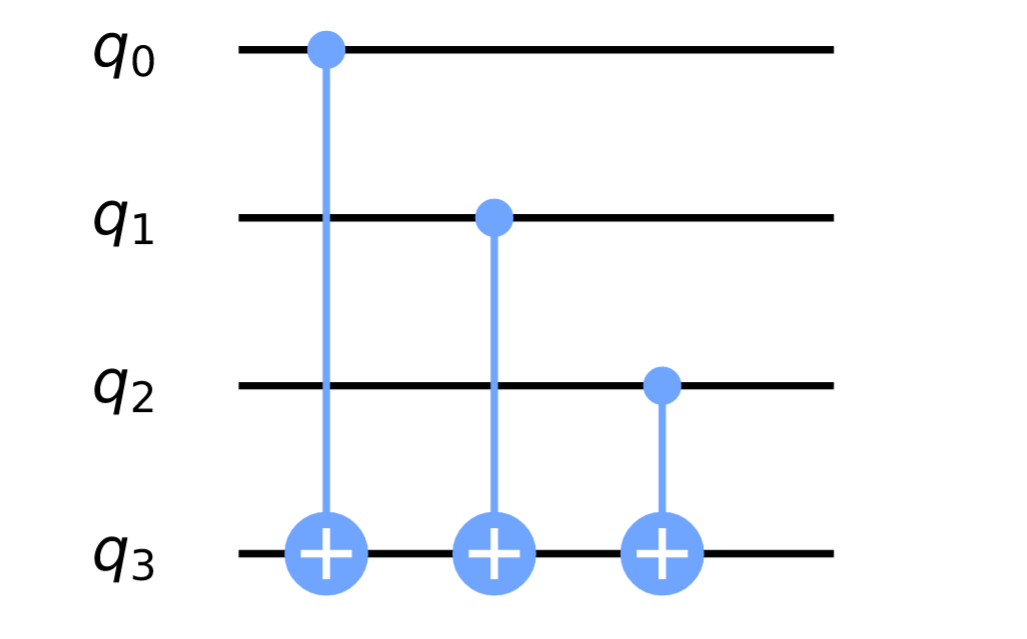
\includegraphics[width=0.8\textwidth]{oraclecon.png}
		\caption{}
	\end{figure}
\end{center}




در تصویر بالا، سه کیوبیت بالا، رجیستر ورودی را تشکیل می دهند و کیوبیت پایین، ثبات خروجی است. در جدول زیر می‌توانیم ببینیم کدام حالت‌های ورودی کدام خروجی را می‌دهند:
\begin{table}[h]
	\centering
	\begin{tabular}{|c|c|}
		\hline
		حالاتی ورودی که به خروجی صفر منجر می‌شوند &  حالاتی ورودی که به خروجی صفر منجر می‌شوند \\ \hline
		000 & 001 \\ \hline
		011 & 100 \\ \hline
		101 & 010 \\ \hline
		110 & 111 \\ \hline
	\end{tabular}
	\caption{This is a simple table.}
\end{table}
ما می توانیم نتایج را تغییر دهیم و در عین حال تعادل آنها را با قرار دادن کنترل های انتخاب شده در X-Gates حفظ کنیم. برای مثال، مدار و جدول نتایج آن را در زیر ببینید:
\begin{center}
	\begin{figure}[ht]
		\centering
		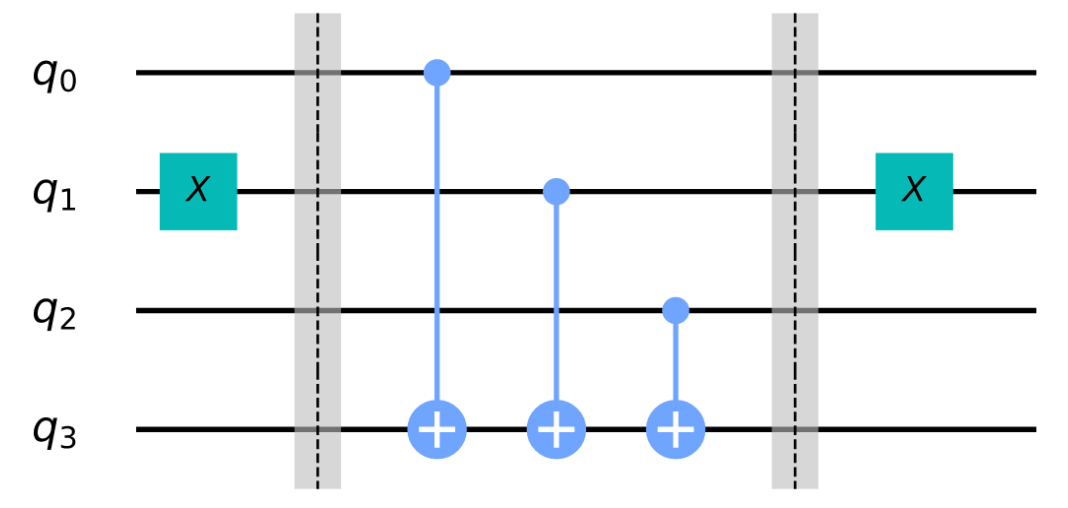
\includegraphics[width=0.8\textwidth]{oraclebalance.png}
		\caption{}
	\end{figure}
\end{center}


\begin{table}[h]
	\centering
	\begin{tabular}{|c|c|}
		\hline
		حالاتی ورودی که به خروجی صفر منجر می‌شوند &  حالاتی ورودی که به خروجی صفر منجر می‌شوند \\ \hline
		001 & 000 \\ \hline
		010 & 011 \\ \hline
		100 & 101 \\ \hline
		111 & 110 \\ \hline
	\end{tabular}
	\caption{This is a simple table.}
\end{table}



% implimentation : https://learn.qiskit.org/course/ch-algorithms/deutsch-jozsa-algorithm
\section{comp vs simulation}
	
% computer vs simulator https://www.youtube.com/watch?v=2qcvgXaDdfU
% https://www.youtube.com/watch?v=0RPFWZj7Jm0	

\chapter{شبیه‌سازی پدیده‌های کوانتومی}
در این بخش قصد داریم به بررسی پروتکل‌های ابتدایی در نظریه‌ی اطلاعات کوانتومی بپردازیم. تمامی این پروتکل‌ها به تعداد کمی کیوبیت نیاز دارند؛ و در آزمایشگاه به صورت تجربی پیاده‌سازی شده‌اند. 
\section{Bell states}
% https://www.youtube.com/watch?v=I0jH1_H3x1o
% pls search about bell eq
در اغلب موارد، سیستم از دو کیوبیت درهمتنیده تشکیل شده‌است. تابع حالت این سیستم‌ها به شکل زیر تعریف می‌شوند:
\begin{center}
	$\vert \psi_{00} \rangle = \frac{1}{\sqrt{2}}(|00\rangle + |11\rangle)$
\end{center}
برای آماده‌سازی این حالت کوانتومی‌، در حالت \lr{$\vert0\rangle$} داریم. با اعمال یک گیت هدامارد روی یکی از کیوبیت‌ها و سپس با کنترل‌ آن با گیت \lr{CNOT}، (به نحوی که کیوبیت دوم هدف قرارگیرد.) می‌توان به یک حالت درهمتنیده رسید. می‌توان این مراحل را به شکل زیر شرح داد:
\begin{center}
	$\vert\psi_{00}\rangle = C_{10}H_{1}\vert00\rangle$
\end{center}

%می‌توان رابطه‌ی بالا را به هریک از حالات $\vert00\rangle, \vert 01\rangl, \vert 10\rangl, \vert 11\rangl$ تعمیم داد:%
\[
\vert\psi_{xy}\rangle = C_{10}H_{1}\vert xy \rangle
\]

از آنجایی که چهار حالت $\vert xy\rangle$ یک مجموعه متعامد هستند و گیت‌های هادامارد و cNOT یکه هستند، چهار حالت درهم تنیده $\vert \psi_{xy}\rangle$ نیز یک مجموعه متعامد هستند، که به نام پایه Bell نامگذاری شده‌اند.  می‌توان رابطه‌ی بالا را یک حالت کلی تعمیم داد:

% read about bell state equation
\begin{center}
$\vert \psi_{xy}\rangle = C10H1X^{x}_{1} X^{y}_{0} \vert00\rangle$\\
\end{center}

\begin{figure}
	\centering
	\begin{subfigure}[b]{}
		\centering
		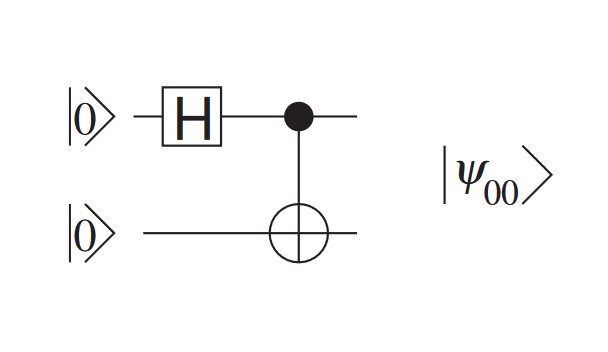
\includegraphics[width=0.2\textwidth]{psi00.png}
		\caption{$y=x$}
		\label{fig:y equals x}
	\end{subfigure}
	\hfill
	\begin{subfigure}[b]{}
		\centering
		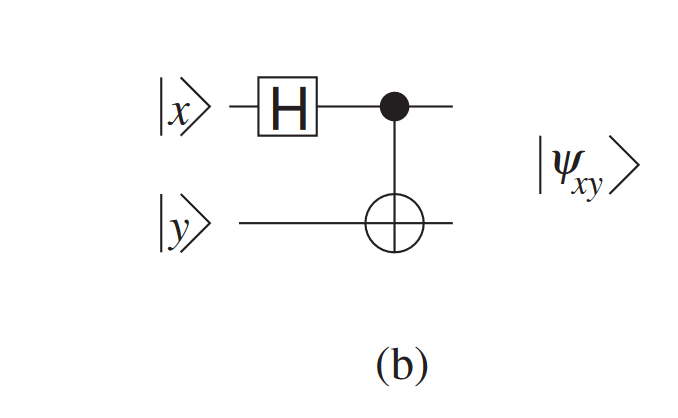
\includegraphics[width=0.2\textwidth]{psixy.png}
		\caption{$y=3\sin x$}
		\label{fig:three sin x}
	\end{subfigure}
	\caption{(a) A circuit that creates the entangled state
		|ψ00〉 = 1√2
		(|00〉 + |11〉) from the unentangled computational-basis
		state |00〉. (b) A circuit that creates the four orthonormal entangled
		Bell states |ψxy〉 from the unentangled computational-basis state |xy〉}
	\label{fig:three graphs}
\end{figure}


درنظر داشته باشید که حالات بل قابل تبدیل به یکدیگرند؛ با کمک رابطه‌ی تعمیم یافته ‌می‌توان از هر حالت بل به حالت $\vert00 \rangle$ رسید.
توضیحات درباره‌ی تبدیلات بنویس

این روابط به شکل‌های متعدد قابل بیان است که از حوصله‌ی بحث خارج است.







\section{entanglement}
\section{super dense coding}


Although an infinite amount of information is needed to specify the state |ψ〉 = α|0〉 + β|1〉 of a single Qbit, there is no way for somebody who has acquired possession of the Qbit to learn what that state is, as we have often noted. If Alice prepares a Qbit in the state |ψ〉 and sends it to Bob, all he can do is apply a unitary transformation of his choice and then measure the Qbit, getting the value 0 or 1. 





After that the state of the Qbit is either |0〉 or |1〉 and no further measurement can teach him anything about its original state |ψ〉. The most Alice can communicate to Bob by sending him a single Qbit is a single bit of information. If, however, Alice has one member of an entangled pair of Qbits in the state |〉 = 1√2 (|0〉|0〉 + |1〉|1〉) (6.15) and Bob has the other, then by suitably preparing her member of the pair and then sending it to Bob, she can convey to him two bits of information.




 She does this by first applying the transformation 1, X, Z, or ZX to her Qbit, depending on whether she wants to send Bob the message 00, 01, 10, or 11. If hers is the Qbit on the left in (6.15) these transform the state of the pair into one of the four mutually orthogonal Bell states (6.5), 
1a |〉 = 1√2 (|0〉|0〉 + |1〉|1〉),
Xa |〉 = 1√2 (|1〉|0〉 + |0〉|1〉),(6.16)
Za |〉 = 1√2 (|0〉|0〉 − |1〉|1〉),
Za Xa |〉 = 1√2 (|0〉|1〉 − |1〉|0〉).



She then sends her Qbit over to Bob. He sends the pair through the controlled-NOT gate Cab , using the Qbit he received from Alice as control, to get
Cab 1a |〉 = 1√2 (|0〉 + |1〉)|0〉,
Cab Xa |〉 = 1√2 (|0〉 + |1〉)|1〉, (6.17)
Cab Za |〉 = 1√2 (|0〉 − |1〉)|0〉,
Cab Za Xa |〉 = 1√2 (|0〉 − |1〉)|1〉,


and then he applies a Hadamard transform to get 
Ha Cab 1a |〉 = |0〉|0〉,
Ha Cab Xa |〉 = |0〉|1〉, (6.18)
Ha Cab Za |〉 = |1〉|0〉,
Ha Cab Za Xa |〉 = |1〉|1〉.



Measuring the two Qbits then gives him 00, 01, 10, or 11 – precisely the two-bit message Alice wished to send. This process of transforming the Bell basis back into the computational basis – i.e. undoing the process (6.3) by which the Bell basis was constructed from the computational basis – and then measuring is called “measuring in the Bell basis.” One can directly demonstrate that this works with circuit diagrams,
without going through any of the analysis in (6.15)–(6.18). 





Suppose that Alice represents the two bits x and y she wishes to transmit to Bob as the computational-basis state |x〉|y〉 of two Qbits (the top two wires, Figure 6.4(a)). If Bob has two Qbits initially in the state |0〉|0〉 (the bottom two wires in Figure 6.4(a)), then the circuit in Figure 6.4(a) gets the two bits to Bob in a straightforward classical way, transforming the state |x〉|y〉|0〉|0〉 on the right to |x〉|y〉|x〉|y〉 on the left by means of direct Qbit-to-Qbit coupling via two cNOT gates. The procedure involves only classical operations on classically meaningful states.




 It gets the two bits from Alice to Bob by explicit interactions between her Qbits and his. It would work equally well for Cbits. One can transform this direct classical procedure into the more exotic quantum protocol by expanding the cNOT gates into products of quantum gates. One first expands one of the C gates into HCZH in Figure 6.4(b). Because Z acting on the control Qbit commutes with C and because C is its own inverse, we can further expand Figure 6.4(b) to Figure 6.4(c). We can then bring the H and C gates on either side of the CZ to the extreme left and right to get Figure 6.4(d).
 
 
 
 
  We can also expand the two C gates on the left of Figure 6.4(d) into the three C gates on the left of Figure 6.4(e), since the action of either set is to flip the target Qbit if and only if the computational-basis states of the two control Qbits are different, while leaving the states of the control Qbits unaltered. Because the state H|0〉 = (1/√2)(|0〉 + |1〉) is invariant under the action of X, the C on the extreme left of Figure 6.4(e) acts as the identity, and Figure 6.4(e) simplifies to Figure 6.4(f). The fact that Figure 6.4(f) has the same action as Figure 6.4(a) contains all the content of the dense-coding protocol. The pair of gates C10H1 on the left of Figure 6.4(f) acts on the state |0〉|0〉 to produce the entangled state (6.15). The bottom Qbit of the pair, Qbit 0, is given to Bob and the upper one, Qbit 1, is given to Alice, who also possesses the upper two, Qbits 2 and 3. 
  
  
  
  
  The pair of gates CZ 31 C21 acts as 1, X, Z, or ZX on Qbit 1 depending on whether the states of Qbits 3 and 2 are |0〉|0〉, |0〉|1〉, |1〉|0〉, or |1〉|1〉. This reproduces the transformation Alice applies to the member of the entangled pair in her possession, depending on the values of the two bits she wishes to transmit to Bob.
  
  
  
   Alice then sends Qbit 1 to Bob. The final pair H1C10 on the right is precisely the transformation (6.18) that Bob performs on the reunited entangled pair before making his measurement, which yields the values x, y that Alice wished to transmit. Like dense coding, many tricks of quantum information theory, including the one we examine next, teleportation, rely on two or more people sharing entangled Qbits, prepared some time ago, carefully stored in their remote locations awaiting an occasion for their use. While the preparation of entangled Qbits (in the form of photons) and their transmission to distant places has been achieved, putting them into entanglement-preserving, local, long-term storage remains a difficult challenge.
\section{Teleport}
isac book
فرض کنید آلیس یک کیوبیت در حالت زیر دارد:
\begin{center}
$\vert \psi \rangle = \alpha\vert 0 \rangle + \beta\vert 1 \rangle $\\	
\end{center}

	کارول ممکن است با اعمال یک عملگر یکه‌ به یک کیوبیت در حالت استاندارد، کیوبیت را از حالت $\vert0\rangle$ به حالت $\vert\psi\rangle$  تبدیل کرده باشد. کارول بدون اعلام نوع عملگر یکه به آلیس،‌ کیوبیت را برای او ارسال می‌کند. 
	حال آلیس می‌خواهد بدون دسترسی داشتن به کیوبیت باب، تغییراتی را در کیوبیت او ایجاد کند؛ این تنها درصورتی ممکن است که کیوبیت باب و آلیس درهمتنیده باشند. هرچند آلیس و باب می‌توانند از طریق راه‌های کلاسیک(نظیر تلفنی صحبت کردن و ...) با یکدیگر ارتباط برقرار کنند؛ ولی نمی‌توانند دسترسی مستقیم به کیوبیت یکدیگر داشته باشند. 
	
	کیوبیت باب را می‌توان به حالت زیر تعریف کرد:
$\vert\phi\rangle = 1/\sqrt{2}(\vert0\rangle \vert0\rangle + \vert1\rangle\vert1\rangle)$ 
	
he no-cloning theorem prohibits duplicating the unknown state
of Alice’s first Qbit, either far away from her or nearby. But it turns
out to be possible for Alice and Bob to cooperate over the telephone
in assigning the state |ψ〉 to Bob’s member of the entangled pair. The
no-cloning theorem is not violated because in doing so Alice obliterates
all traces of the state |ψ〉 from either of her own Qbits. The process –
called teleporting the state from Alice to Bob – also eliminates the en-
tanglement Alice and Bob formerly shared. For each shared entangled
pair, they can teleport just a single 1-Qbit state. The term “teleporta-
tion” emphasizes that the state assignment acquired by Bob’s Qbit no
longer applies to Alice’s; it has been transported from her Qbit to his.
Here is how teleportation works. Alice’s first Qbit and the entangled
pair she shares with Bob are characterized by the 3-Qbit state
|ψ〉a |〉ab = (α|0〉a + β|1〉a
) 1√2
(|0〉a |0〉b + |1〉a |1〉b
), (6.21)
where I have given the state symbols for the Qbits in Alice’s and Bob’s
possession subscripts a and b . To teleport the unknown state of her
Qbit to Bob’s member of the entangled pair, Alice first applies a cNOT
gate, using her first Qbit in the state |ψ〉 as the control and her member
of the shared entangled pair as the target. This produces the 3-Qbit
state
α|0〉a 1√2
(|0〉a |0〉b + |1〉a |1〉b
) + β|1〉a 1√2
(|1〉a |0〉b + |0〉a |1〉b
).
(6.22)
Next she applies a Hadamard transformation H to her first Qbit, giving
all three Qbits the state
α 1√2
(|0〉a + |1〉a
) 1√2
(|0〉a |0〉b + |1〉a |1〉b
)
+ β 1√2
(|0〉a − |1〉a
) 1√2
(|1〉a |0〉b + |0〉a |1〉b
)
= 1
2 |0〉a |0〉a
(α|0〉b + β|1〉b
) + 1
2 |1〉a |0〉a
(α|0〉b − β|1〉b
)
+ 1
2 |0〉a |1〉a
(α|1〉b + β|0〉b
) + 1
2 |1〉a |1〉a
(α|1〉b − β|0〉b
). (6.23)
Now Alice measures both Qbits in her possession. (As remarked
in Section 6.4, such an application of cNOT and Hadamard gates,
immediately followed by measurement gates, is called “measuring in
the Bell basis.”) If the result is 00, Bob’s Qbit will indeed acquire the
state |ψ〉 originally possessed by Alice’s first Qbit (whose state would
then be reduced to |0〉). But if the result of Alice’s measurement is 10,
01, or 11 then the state of Bob’s Qbit becomes
α|0〉b − β|1〉b , α|1〉b + β|0〉b , or α|1〉b − β|0〉b . (6.24)
In each of these three cases there is a unitary transformation that re-
stores the state of Bob’s Qbit to Alice’s original state |ψ〉. In the first
case we can apply Z (which leaves |0〉 alone but changes the sign of |1〉),
in the second case, X (which interchanges |0〉 and |1〉), and in the third
case, ZX.
6 . 5 TE L E P O R T A T I O N 151
So all Alice need do to transfer the state of her Qbit to Bob’s member
of their entangled pair is to telephone Bob and report to him the results
of her two measurements. He then knows whether the state has already
been transferred (if Alice’s result is 00) or what unitary transformation
he must apply to his member of the entangled pair in order to com-
plete the transfer (if Alice’s result is one of the other three.) Note the
resemblance to quantum error correction: by making a measurement
Alice acquires the information needed for Bob to reconstruct a partic-
ular quantum state, without anybody acquiring any information about
what the state actually is.
This appears to be remarkable. A general state of a Qbit is described
by two complex numbers α and β that take on a continuum of values,
constrained only by the requirement that |α|2 + |β|2 = 1. Yet, with the
aid of a standard entangled pair, whose state does not depend on α and
β, Alice is able to provide Bob with a Qbit described by the unknown
state, at the price of only two bits of classical information (giving the
results of her two measurements) and the loss of the entanglement of their pair.






But of course the teleportation process does not communicate to Bob the information that can be encoded in α and β. Bob is no more able to learn the values of α and β from manipulating his Qbit, now assigned the state |ψ〉, than Alice was able to do when it was her Qbit that was assigned the same state |ψ〉. On the other hand Alice’s state could be produced at a crucial stage of an elaborate quantum computation, and its transfer to Bob could enable him to continue with the computation on his own far-away quantum computer, s  one can achieve a nontrivial objective by such teleportations. Like dense coding, teleportation can also be constructed by manipulating an elementary classical circuit diagram, without going through any of the analysis in (6.21)–(6.24). Figure 6.5(a) shows a circuit that exchanges the state |ψ〉 = |x〉 of Alice’s Cbit with the state |0〉 of Bob’s Cbit, regardless of whether x = 0 or 1. The transfer is achieved by direct physical coupling between the two Cbits. As a linear quantum circuit it continues to perform this exchange for arbitrary superpositions, |ψ〉 = α|0〉 + β|1〉. The entire teleportation protocol can be constructed by appropriately expanding the two gates in Figure 6.5(a), with the aid of an ancillary Qbit. The aim of the expansion is to eliminate the direct interaction between Alice’s and Bob’s Qbits through the two cNOT gates in Figure 6.5(a), in favor of the telephoned message from Alice to Bob, and the interaction necessary to produce their shared pair of entangled Qbits (which can take place well before Alice has even acquired her Qbit in the state |ψ〉).





In Figure 6.5(b) an ancillary Qbit, not acted upon throughout the process, is introduced in the state |φ〉 = H|0〉 = 1√2 (|0〉 + |1〉). (6.25) In Figure 6.5(c) the identities X = HZH and 1 = HH have been used to rewrite the cNOT gate on the right of Figure 6.5(b), and an additional cNOT gate has been added on the left, which acts as the identity, since X acts as the identity on the state H|0〉. Figure 6.5(d) follows from Figure 6.5(c) because the action of CZ is independent of which Qbit is the control and which the target, and because the two cNOT gates on the left of Figure 6.5(c) have exactly the same action as the three cNOT gates on the left of Figure 6.5(d): acting on the computational basis, both sets of gates apply X on both of the bottom two wires if the state of the top wire is |1〉 and act as the identity if the state of the top wire is |0〉. Figure 6.5(e) follows from Figure 6.5(d) if we write the |φ〉 on the left of Figure 6.5(d) as H|0〉 and explicitly write the |0〉 on the right of Figure 6.5(d) as H|φ〉. But Figure 6.5(e) is an automated version of teleportation. To relate it to ordinary teleportation, introduce mea- surements of the upper two Qbits after the circuit of Figure 6.5(e) has acted, as in Figure 6.5(f). Their effect is to collapse the states of each of the two upper wires randomly and independently to |0〉 or |1〉. But as noted in Section 3.6, measurement of a control Qbit commutes with any operation controlled by that Qbit, so the measurement gates can be moved to the positions they occupy in Figure 6.5(g). Figure 6.5(g) is precisely the teleportation protocol. The two gates on the left transform the two lower Qbits into the entangled state (6.20). The subsequent applications to the top two Qbits of cNOT followed by H followed by two measurement gates are precisely Alice’s “measurement in the Bell basis.” Since Alice knows the outcomes of the measurements, she knows whether the subsequent cNOT and CZ gates will or will not act, and she can replace these physical couplings by a phone call to Bob telling him whether or not to apply X and/or Z directly to his own Qbit. Figure 6.6 demonstrates that entanglement can also be teleported. The figure reproduces parts (b), (e), and (g) of Figure 6.5 with three changes. (1) A bar representing n Qbits in the n-Qbit state |〉i has been added above each part of the figure. No operations act on these additional Qbits. (2) The state to be teleported has been given a subscript i so it is now one of several possible states |ψi 〉. (3) Because of the linearity of the unitary gates we may sum over the index i . The effect of the circuit is to transfer participation in the entangled state ∑ i |i 〉|ψi 〉 from the third wire from the bottom to the bottom wire. So even if Alice’s Qbit has no state of its own but is entangled with other Qbits, Alice can use the same protocol to teleport its role in the entangled state over to Bob’s Qbit. The result is that Bob’s Qbit becomes entangled in exactly the same way Alice’s was, and Alice’s Qbit becomes entirely unentangled.
1
\newpage
how to determine a oracle\\
	
	
	
	
% https://learn.qiskit.org/course/ch-algorithms/quantum-circuits
	
	
	
\end{document}